\section{Introduction}
\label{sec:introduction}

The main purpose of the project is to use a unified analytics engine (Apache Spark) to compare how clustering works with machine learning and how the technology works itself. As we worked before in projects of Machine Learning, we think it would be interesting to work with distributed machine-learning framework.


In 2008, approximately,the basis for creating this technology appeared, Hive and HBase, which are two tools of the Hadoop ecosystem.  
Spark was founded at UC Berkeley in 2009, it was born practically from a Google paper and from there it evolved, going through the mapreduce processes.



\noindent
\begin{figure}[h]
	\centering
	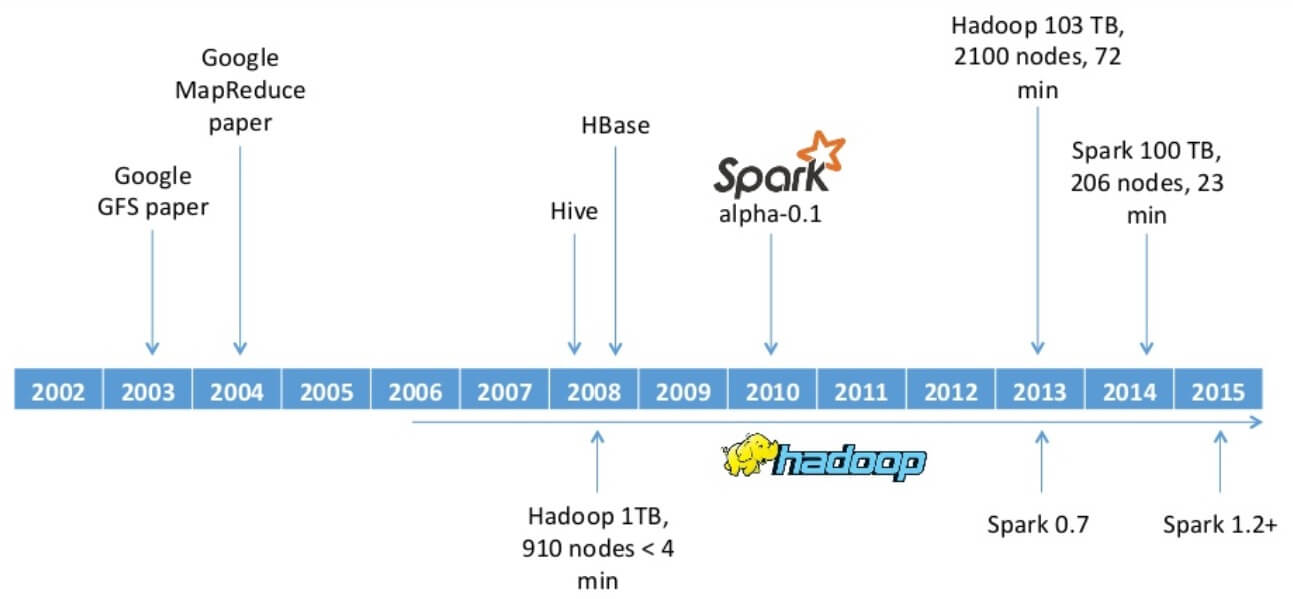
\includegraphics[scale=0.3]{figs/TimelineSpark.jpg}
	\caption{Apache Spark Development Timeline}
	\label{fig:timeline}
\end{figure}

Comparing this technology with others, for example with sklearn, the most well-known library for machine learning porpoises, we are satisfied with our results because the sklearn library is even not able to load big datasets. In addition we are satisfied with the clustering management, it is 60 \% faster than without clustering management. \\*

\noindent

This rest of this report is organised as follows:

\begin{itemize}


\item Section~\ref{sec:background} gives an overview of the key concepts and the architecture.

\item Section~\ref{sec:prototype} gives a view of the prototype and its implementation

\item Section~\ref{sec:experiments} gives an explanation of the test-bed environment used and the results of the experiments

\item Section~\ref{sec:conclusion} gives a conclusion about the main concepts that we appreciated from this technology.

\end{itemize}
\noindent